\documentclass{sig-alt-release2}
\usepackage{url}
\usepackage{color}
\usepackage{graphics,graphicx}

\usepackage{epsfig}
\usepackage{epstopdf}

\usepackage{colortbl}
\usepackage{multirow}
\usepackage{booktabs}
\usepackage{ifthen}  

\begin{document}
\newcommand{\todo}[1]{\textcolor{red}{#1}}
\def\newblock{\hskip .11em plus .33em minus .07em}

\conferenceinfo{DIM3} {2012, Glasgow, UK} 
\CopyrightYear{2012}
\clubpenalty=10000
\widowpenalty = 10000

\title{{iHero Specification}}

\numberofauthors{4}
\author{
  \alignauthor 
  Gary Blackwood \textit{0906796b}\\
  Ian Scott \textit{0901475s}\\
  John Dennis \textit{0907383d}\\
  Paul Moore \textit{0901723m}\\
  \affaddr{eKitchen}\\
  \affaddr{DIM3}\\
}
\maketitle

\begin{abstract}
iHero is a social media app that allows the general public to submit reports of incidents and disasters at their current location. Emergency service personnel will then be able to view the reports as submitted by the public. The idea is that an event will only be submitted once by the first user, and other users can vote up or down the credibility of the event and comment on the event to provide more detail.

The idea is that we are collating all the data in one place - as opposed to Emergency Services having to trawl through Twitter feeds and Facebook pages. It is in no way designed to replace calling the emergency services directly, but instead as a tool to aid them. iHero is aimed at all of the general public through smartphone optimisation for on the go reporting as well as desktop browsing.
\end{abstract}

\begin{table}[!ht]
  \caption{User group functionality.}
  \label{user-table}
  \begin{center}
    \begin{tabular}{ | p{3cm} | p{3cm} | }
      \hline
      General Public & Emergency Services \\
      \hline
      Required & Required \\
      \hline
      The ability to submit a report with a title/description, location and seriousness rating. List recent incidents to the user and allow them to be voted up or down. 
      &
      View a list of submitted incident reports. Log in and update or delete incidents. \\
      \hline
      Desired & Desired \\
      \hline
      Allow users to upload photos and videos along with their submission. If the submission is made from a mobile device, pull the GPS location from it. ``Did you mean this fire on xyz street?'' feature to prevent many reports of the same incident.
      &
      View the incidents on a map. \\
      \hline
    \end{tabular}
  \end{center}
\end{table}


\section{Aim of Application}
iHero is a web application that will allow users to upload reports of incidents that occur in the real world. The main aim of this service is to provide information about incidents in a clear and concise way that can be used by emergency services. To sort the most important reports, users can give a rating of how serious the incident is when they submit it. This combined with allowing all users to vote submissions up or down should filter the most urgent incidents to the top of the list.

The two user groups that will interact with our system will be the emergency services and the general public. These two groups will use the system in different ways. Both will be able to view lists of recent incidents, the general public will have the option to up or down vote these submissions based on their credibility and urgency where as the emergency services only need to view the lists. The general public also have the added functionality of being able to report incidents.

We aim to implement as much the required functionality as possible. The main constraint on this project is time and resources. We have limited time to implement the system and as a team of four people we feel the functionality is reasonably complex.                            

The finished application should also meet a number of non functional requirements. The website should be easily usable, we will do this by making a simple, clean client interface that emphasizes recognition over recall. It must also be reliable as the data we are receiving could potentially be very important. It is our aim to optimize the website for mobile devices because this will be where most of the incident reports come from. Doing this also allows the emergency services to locate incidents close to them when they are out and about.

\section{Client Interface}
Our interface must be minimal and clean. iHero is optimised to be used on smartphones and tablet devices, as well as by standard desktop browsers, through the use of a responsive CSS implementation from Twitter Bootstrap. The website reacts to the screen size of the device being used. If the device has a smaller screen width the layout of the website will adapt to fit the users environment and provide them with the best possible experience.

We provide our brand logo in the customary top left position to provide feedback to the user that they have arrived at the correct location (Label 1). The users may be in a state of shock or distress when using our system. As can be seen, from the wireframe below of the main screen, we ask for minimal amounts of required field data (Labels 3 through 5). Simply the event or disaster title, the exact location and a judgement of the seriousness rating. If using a mobile phone the application will record geolocation data about the position the user is currently at but provide the user with a section to give more precise detail. We think this is enough data to allow other users to be able to verify an event. We provide a button to allow more data to be input should the user wish to give us more if the circumstances and surroundings should permit them to.

If the user opts to input more information the form will expand and allow them to upload a picture, video, extra details including the time of the incident, a box to give more details and also a tags field to aid searches.

The emergency services have a different view, accessible by the button labelled ``Emergency Services Login'' (Label 6) This will provide a listing of all the incidents and events, sortable on different categories. Emergency services will have the right to delete rogue information that they know to be untrue or exaggerated.

This easy, appealing and simple user interface allows the user to quickly fill out the emergency report and submit it to the iHero system - no complicated forms, a few select number of fields, and all in one page.

\begin{figure}
  \caption{Submit Incident View}
  \begin{center}
    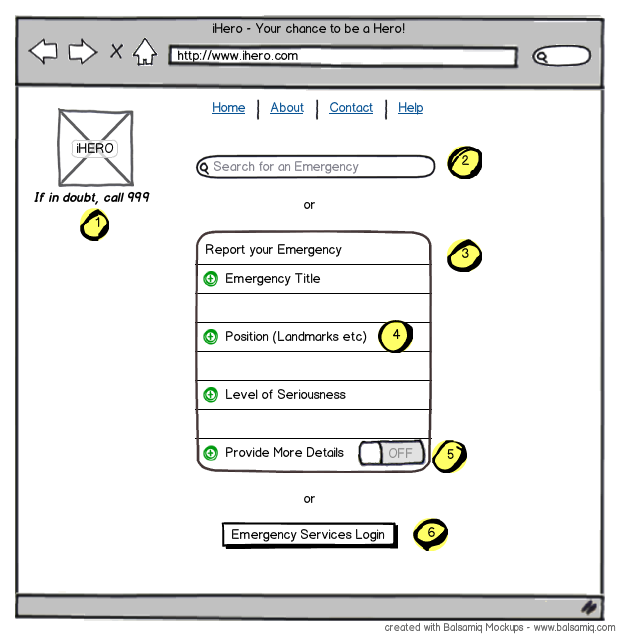
\includegraphics[scale=0.4]{img/1.png}
  \end{center}
\end{figure}

\begin{enumerate}
  \item Logo and links to other parts of the site. This appears on each page and allows for easy navigation around the application.
  \item Search bar - allows users to search for incidents.
  \item Form for submitting an incident.
  \item Location field, the information given here is passed to the google maps API by the middleware.
  \item Space for extra details such as a description, photos or video.
  \item Link to emergency services log in.
\end{enumerate}

For the current incidents view - the template layout will be consistent with the form to report an incident however the middle section will change to a list view. This will allow people to see what has already been reported, to get and or add more info (for each incident - see label 3) and also to vote up or down the validity of the report.
The emergency services will be able to login to the system and an extra part will be added to this page to allow them to remove invalid reports and to give feedback to people on the current situation at that incident.

\begin{figure}
  \caption{Incident List View}
  \begin{center}
    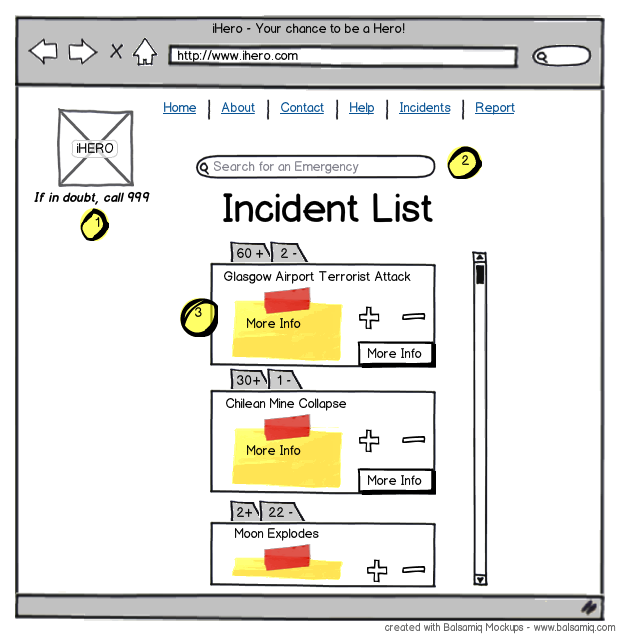
\includegraphics[scale=0.4]{img/5.png}
  \end{center}
\end{figure}

\begin{enumerate}
  \item Logo and links to other parts of the site. This appears on each page and allows for easy navigation around the application.
  \item Search bar - allows users to search for incidents.
    \item List of incidents - each incident can be voted on and is expandable. Showing the title, description, location, a map view and the number of up and down votes.
\end{enumerate}

\subsection{Technologies}

\subsubsection{HTML}
It is anticipated we will use HTML5 or XHTML for this project. Using HTML5 brings us to the forefront of technology and provides us with the most up to date features for web based applications - however not all browsers can support this yet. Most smartphone browsers can handle the new features of HTML5     but desktop browsers are not all up to date. This is where XHTML can be used for backwards compatibility, however this is more complex than basic HTML.

\subsubsection{CSS (Twitter Bootstrap)}
We plan to make use of the Twitter Bootstrap CSS framework to give a clean, familiar styling to our user interface. Using CSS (Cascading Style Sheets) is good programming practice as it removes all styling from the HTML code. This means that the style can change without having to edit the content, and vice versa. This seperates out concerns, as the style and content are independent of each other.

\subsubsection{jQuery and JavaScript}
We will also use jQuery to provide active content to our site, such as expanding the more details field if the user wishes to do so.

\section{Application Architecture}

\begin{figure}[!ht]
  \caption{iHero tiered architecture.}
  \begin{center}
    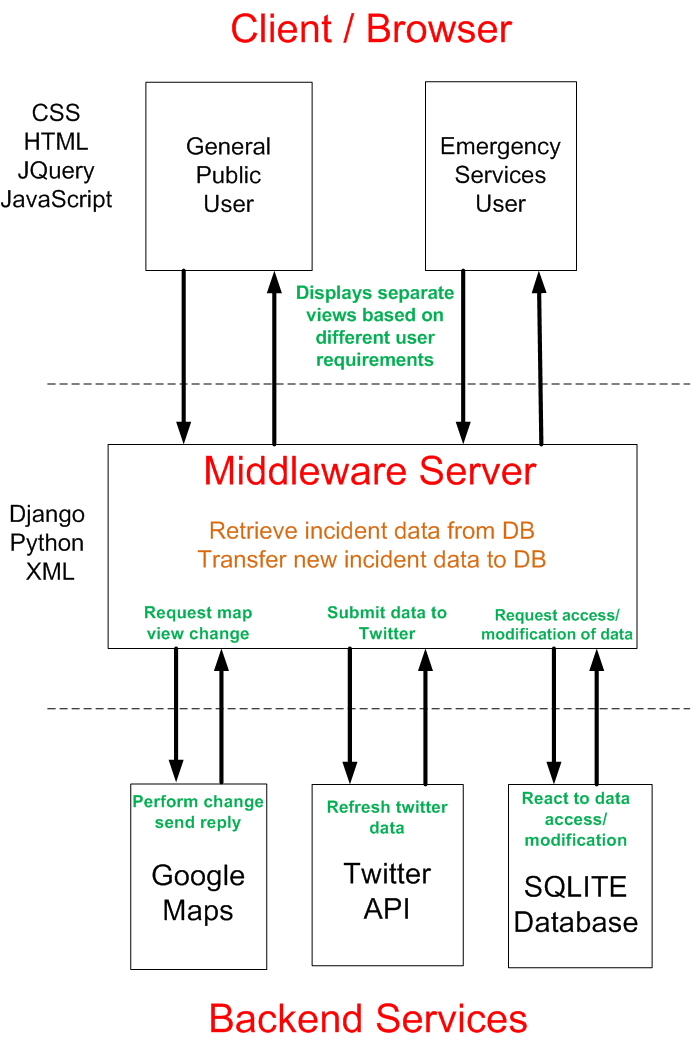
\includegraphics[scale=0.3]{img/2.png}
  \end{center}
\end{figure}

\subsection{Client/Browser}

\begin{itemize}
\item    Provides the interface for users to report an incident.
\item    Presents already reported incidents to the user.
  \begin{itemize}
  \item        Time.
  \item        Location.
  \item            Also presented in a map view.
  \item        Description.
  \end{itemize}
\item    Presents data in a structured and organised way using CSS.
\end{itemize}

\subsection{Middleware}

\begin{itemize}
\item    Acts as a receiver of user incident data entries from the Client Tier.
  \begin{itemize}
  \item        Passes this data on to the Backend Server (Database).
  \end{itemize}
\item    Receives queries from the Client tier. Does not anyone have a copy of 
  \begin{itemize}
  \item        Extracts required data from the Backend server in response to these queries.
  \end{itemize}
\end{itemize}

\subsection{Backend}

The backend services are comprised mainly of SQLITE, responsible for data query replies, data organisation and the storage of indicent data. The backend also contains communication points with Google Maps and Twitter.

\begin{itemize}
\item    Provides the storage of incident data using the SQLITE database.
\item    Replies to data queries passed on by the Middleware Server.
\end{itemize}

\subsection{Data Model}

\begin{center}
  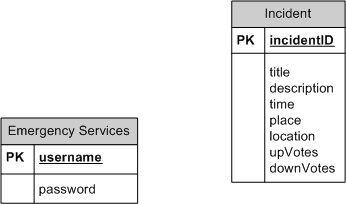
\includegraphics[scale=0.5]{img/4.png}
\end{center}

\begin{itemize}
\item    Emergency services have their username and passwords stored
\item Incidents have the following attributes: ID, title, description, time, location, upvotes, downvotes.
\end{itemize}

\subsection{Seperation of Concerns}

Our design has enabled a change in one tier to be independent from other tiers using standardised communication.

\newpage
\section{Message Passing}

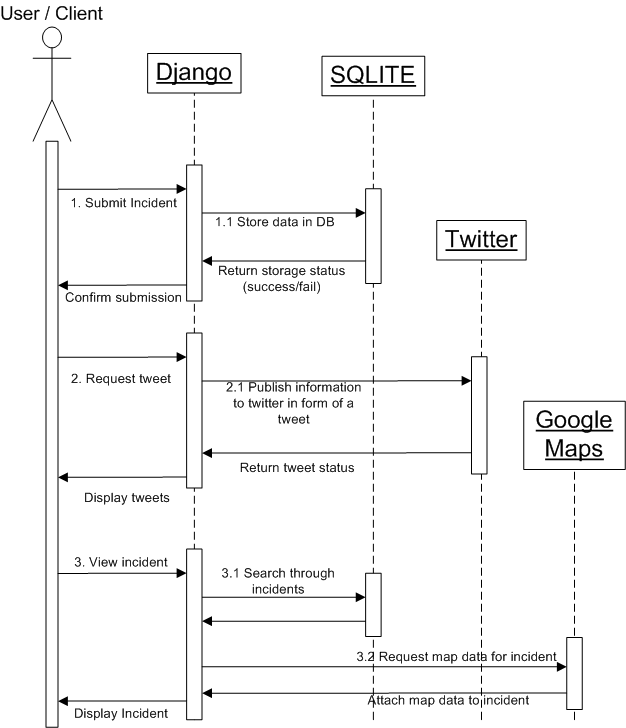
\includegraphics[scale=0.4]{img/3.png}

\begin{enumerate}
\item    User reports an incident, entering the time, location and description of the incident.
\item    Client Tier sends data of reported incident, or request for user to view another incident.
\item    Middleware Server communicates this query to the database in the Backend services and awaits a reply, or requests for new incident data to be stored in the database.
\item    Backend Services records new data and updates the database. Returns a refreshed state for the Middleware to provide to the Client Tier.
\item    Middleware provides new data to Twitter in the form of a tweet.
\item    Twitter API returns results of any queries from the Client Tier via Middleware.
\item    Middleware returns refreshed data back to the Client.
\item    Client displays up-to-date reflection of incident data.
\end{enumerate}

\subsection{Twitter}

\subsubsection{Authentication [POST]}

Users will be able to log in to iHero using their existing
Twitter accounts. The Twitter API provides authentication
functionality OAuth that makes this possible. To authenti-
cate a user, an request token must be obtained.

\tiny
\begin{verbatim}
POST /oauth/request_token HTTP/1.1
User-Agent: themattharris' HTTP Client
Host: api.twitter.com
Accept: */*
Authorization:
OAuth oauth_callback="http%3A%2F%2Flocalhost%2Fsign-in-with-twitter%2F",
oauth_consumer_key="cChZNFj6T5R0TigYB9yd1w",
oauth_nonce="ea9ec8429b68d6b77cd5600adbbb0456",
oauth_signature="F1Li3tvehgcraF8DMJ7OyxO4w9Y%3D",
oauth_signature_method="HMAC-SHA1",
oauth_timestamp="1318467427",
oauth_version="1.0"
\end{verbatim}
\normalsize

If the response received is successful, the next step is to
redirect the user to Twitter so that they may log in using
the information received in the previous step.

\tiny
\begin{verbatim}
https://api.twitter.com/oauth/authenticate?oauth_token=NPcudxy0yU5T3tBzho7iCotZ3cnetKwcTIRlX0iwRl0
\end{verbatim}
\normalsize

Finally, the log in request token is converted to an access
token that is stored throughout the user session.

\tiny
\begin{verbatim}
Authorization: OAuth oauth_consumer_key="cChZNFj6T5R0TigYB9yd1w",
oauth_nonce="a9900fe68e2573b27a37f10fbad6a755",
oauth_signature="39cipBtIOHEEnybAR4sATQTpl2I%3D",
oauth_signature_method="HMAC-SHA1",
oauth_timestamp="1318467427",
oauth_token="NPcudxy0yU5T3tBzho7iCotZ3cnetKwcTIRlX0iwRl0",
oauth_version="1.0"
Content-Length: 57
Content-Type: application/x-www-form-urlencoded
oauth_verifier=uw7NjWHT6OJ1MpJOXsHfNxoAhPKpgI8BlYDhxEjIBY
\end{verbatim}
\normalsize

\subsubsection{Search [GET]}

The Twitter API provides functionality that allows us to
search tweets for those related to a particular incident. The
service recieved HTTP GET requests in the following for-
mat:

\small
\begin{verbatim}
http://search.twitter.com/search.json?rrp=1&q=incidentName
\end{verbatim}
\normalsize

This request will return, in JSON format, tweets related
toincidentName and display them one result per page.

\begin{verbatim}
{"results":
[{"from_user_id_str":"04934854",
"from_user":"user1234",
"created_at":"Tue, 04 Jan 2012 09:32:15+0000",
"text":"The Boyd Orr is on fire!",
"id":39474522797714328,
}]}
\end{verbatim}

\section{Maps}

Using location data provided by a user or their current lo-
cation we can display and update maps related to incidents.
Using the Google Maps API this can be done as follows:

\tiny
\begin{verbatim}
<!DOCTYPE html>
<html>
<head>
<meta name="viewport" content="initial-scale=1.0, user-scalable=no" />
<style type="text/css">
html { height: 100% }
body { height: 100%; margin: 0; padding: 0 }
#map_canvas { height: 100% }
</style>
<script type="text/javascript"
src="http://maps.googleapis.com/maps/api/js?key=YOUR_API_KEY&sensor=SET_TO_TRUE_OR_FALSE">
</script>
<script type="text/javascript">
function initialize() {
var myOptions = {
center: new google.maps.LatLng(-34.397, 150.644),
zoom: 8,
mapTypeId: google.maps.MapTypeId.ROADMAP
};
var map = new google.maps.Map(document.getElementById("map_canvas"),
myOptions);
}
</script>
</head>
<body onload="initialize()">
<div id="map_canvas" style="width:100%; height:100%"></div>
</body>
</html>
\end{verbatim}
\normalsize

This example displays a map centered on Sydney, Aus-
tralia. To update or change the location we use the data
provided by the user and update the following:

\begin{verbatim}
center = new google.maps.LatLng( lat, long )
\end{verbatim}

\newpage
\section{Design Revision / Feedback}
The main theme of the feedback on our specification report was of small changes to increase the clarity of our design. A few people noted that our required functionality seemed ambitious and how we referred to ``desired functionality'' later on in the document when we had never specified it to begin with. It quickly became clear that when transferring our report to LaTeX the ``desired functionality'' heading was omitted. A lack of labels and titles on diagrams was also brought up, and our peers questioned the ER diagram.  One reviewer wanted a design decision explained, asking ``The difference between CSS and CSS(Twitter Bootstrap) is not explained, why did you choose the twitter bootstrap over the original?''. Another person commented that the voting system could be abused.

We valued our peers feedback so we took on board their opinions and made some changes to our report. To clear up the required vs. desired confusion, a table that clearly lays out the functionality was added. Titles and labels were added to wireframe diagrams to make them easier to understand. Based on feedback from one reviewer, who said that the ``seriousness rating'' field for an incident was pointless as most people would be biased and mark their incident as the most important, we agreed with this and chose to leave this out. This leaves the up and down votes as the main indicator of an incidents importance. A few more small changes were made in the specification report to increase clarity. Another good bit of feedback we received was to have a ``most recent'' view, we changed our design to give users the option to view incidents in the last day,week month or all time. The point about Twitter Bootstrap has also been further explained highlighting its usefulness over creating our own CSS stylesheets

The feedback has been helpful, fresh sets of eyes have been able to identify parts of our design that did not make sense or needed better explanation. Decisions that were obvious ones for us were not to others looking at our project, this meant we did not fully explain everything that we were planning to include and forced us to provide more detail in our descriptions. The process of peer review at this stage in development was very useful as it happened before implementation started. This meant that any major changes that needed to be made would not undo any work already spent coding.

\newpage
\section{Implementation Notes}
All of the required functionality specified in the ``Aims of the Application'' section of this document has been implemented. This is true of both the general public and emergency services user groups. Everyone is able to view a list of recent incidents when they first arrive at the site. Each item on the list is expandable and shows the title, a description, location and the votes received. These incidents can be voted up or down and are ordered by net vote. The user can also filter on submission date to remove older incidents from the view. The general public can submit an incident report from the submit page. Emergency Services are also able to log in and delete incidents or edit them to mark them as dealt with. One of our aims was to optimize the application for mobile devices, this allows users to submit incidents as they see them when they are out and about, obviously this also lets emergency service users react to incidents local to them. The site scales down to fit mobile screens, the navigation links at the top are replaced by a button that when clicked will display all the navigation links, search bar and log in fields.

An attempt was made to implement some of the desired functionality too,  Emergency Services should be able to view incidents on a map. This works to an extent, for each incident; a google map and street view image are shown. However, they are not all brought together on one big map that would allow emergency service users to search by location. One fairly big flaw is that there is no restriction on how many times a person can vote on an incident, this could be abused to give incidents artificial positions on the list. Also, if a failed attempt is made to log in to the admin page, users are redirected to the Django log in page as opposed to telling the user there was an error and staying on our site. Another known issue is that the images pulled from google street view may not be useful at all, sometimes there will not be an image available and if there is, it may be showing a building on the other side of the street for example.

The main constraint on developing this application has been time. Although it is currently in a working state we have plans for future development. The most pressing issue is to fix voting, so that users can only vote once on an incident and also use AJAX to handle the votes so that there is no need to reload the whole page after submitting a vote. To further improve iHero the next steps are to implement more of the desired functionality. Allowing users to automatically submit their GPS location details from mobiles would speed up the submission process and handling photos and video uploads would benefit emergency services by giving them a more detailed picture of the situation. On top of that we plan to let users add to other incidents with comments, photos and videos when the application recognises that the incident they are trying to submit is already in the database. We also plan to create individual administration accounts for the emergency services, for example this would mean the fire brigade could not see, and therefore edit, the police or ambulance incidents on the admin pages. This reduces the volume of information displayed to the emergency responders and decreases the end response time of mobilising the emergency services to the incident.. These additions would further improve the service offered by iHero.

\newpage
\section{Reflective Summary}
Developing this application has taught us just how useful frameworks and APIs can be. Reusing code from other sources through such as the Google Maps API and Twitter Bootstrap drastically speeds up the development process to get the site into a working state. This reduces boiler plate code and makes the code easier to read, and therefore easier to maintain. The Django framework let us set up our models and get the site running very quickly. Django provided the admin functionality that lets emergency services log in, remove and edit incidents. Obviously this made implementing the emergency services basic functionality very easy so we could use the time saved to work on more complex features of the website. We did not feel that the Django and Twitter frameworks hindered us in any way as we were able to implement a good amount of functionality without much trouble. By using Twitter Bootstrap we fully seperated our concenrns in the design of the website, as this allowed us to customise the CSS in one file, freeing us from having in-line or embedded style blocks.The same holds true for the JavaScript and jQuery involved in the site.

One of the main problems we faced was the learning curve of the django framework we used. This framework was new to all of us so we had to spend more time researching than implementing which limited how much functionality we could implement in the short period of time we had. The major achievements of the project are that we managed to provide all of the required functionality specified in the original report, and we have done so in what we believe to be a user friendly and efficient way. A lot has been learned about the variety of technologies used to develop the application. We feel that iHero is in a state where it could genuinely be used to aid the emergency services in their work. 

\section{Acknowledgements}
Our thanks to the lecturers and demonstrators for their comments and suggestions. And our thanks to the peer reviewers for their feedback.

\begin{thebibliography}{9}

\bibitem{jakob1}
  Jakob Nielsen,
  \emph{Heuristics for User Interface}.

\bibitem{jakob}
  Django Documentation,
  \emph{https://www.djangoproject.com/}.

\bibitem{twitter}
  Twitter Bootstrap,
  \emph{http://twitter.github.com/bootstrap/index.html}.

\bibitem{Stack}
  StackOverflow,
  \emph{http://stackoverflow.com/}.

\end{thebibliography}

\end{document}
